% \documentclass{article}
% %\usepackage[english]{babel}%
% \usepackage{graphicx}
% \usepackage{tabulary}
% \usepackage{tabularx}
% \usepackage[normalem]{ulem}
% \usepackage{cancel}
% \usepackage{tikz} 
% \usepackage{pdflscape}
% \usepackage{colortbl}
% \usepackage{lastpage}
% \usepackage{multirow}
% \usepackage{enumerate}
% \usepackage[shortlabels]{enumitem}
% \usepackage{color,soul}
% \usepackage{pdflscape}
% \usepackage{hyperref}
% %\usepackage[table]{xcolor}
% \usepackage{rotating}
% \usepackage{amsmath}
% \usepackage{fixltx2e}
% \usepackage{framed}
% \usepackage{mdframed}
% \usepackage[T1]{fontenc}
% \usepackage[utf8]{inputenc}
% \usepackage{textcomp}
% \usepackage{siunitx}
% \usepackage{ifthen}
% \usepackage{fancyhdr}
% \usepackage{gensymb}
% \usepackage{newunicodechar}
% \usepackage[document]{ragged2e}
% \usepackage[margin=1in,top=1.1in,headheight=57pt,headsep=0.1in]
% {geometry}
% \usepackage{ifthen}
% \usepackage{fancyhdr}
% \everymath{\displaystyle}
% \usepackage[document]{ragged2e}
% \usepackage{fancyhdr}
% \everymath{\displaystyle}
% \usepackage{empheq}

% \usepackage[most]{tcolorbox}

% \usepackage{booktabs} % Required for nicer horizontal rules in tables


% \usepackage{enumitem}

% %\usepackage[table,xcdraw]{xcolor}
% \usetikzlibrary{arrows}
% \linespread{2}%controls the spacing between lines. Bigger fractions means crowded lines%
% %\pagestyle{fancy}
% %\usepackage[margin=1 in, top=1in, includefoot]{geometry}
% %\everymath{\displaystyle}
% \linespread{1.3}%controls the spacing between lines. Bigger fractions means crowded lines%
% %\pagestyle{fancy}
% \pagestyle{fancy}
% \setlength{\headheight}{56.2pt}

% \definecolor{myblue}{rgb}{.8, .8, 1}
% \newcommand*\mybluebox[1]{%
% \colorbox{myblue}{\hspace{1em}#1\hspace{1em}}}

% \chead{\ifthenelse{\value{page}=1}{\includegraphics[scale=0.3]{SCC}\\ \textbf \textbf Wastewater Constituents Analysis \& Laboratory Methods}}
% \rhead{\ifthenelse{\value{page}=1}{}{}}
% \lhead{\ifthenelse{\value{page}=1}{}{Wastewater Constituents Analysis \& Laboratory Methods}}
% \rfoot{\ifthenelse{\value{page}=1}{Module 1: WATR 048 - Spring 2019}{Module 1: WATR 048 - Spring 2019}}

% \lfoot{Shabbir Basrai}
% \cfoot{Page \thepage\ of \pageref{LastPage}}
% \renewcommand{\headrulewidth}{2pt}
% \renewcommand{\footrulewidth}{1pt}
% \begin{document}
% %\begin{empheq}[box=\mybluebox]{align}
% %a&=b\\
% %E&=mc^2 + \int_a^a x\, dx
% %\end{empheq}

% \newlist{steps}{enumerate}{1} % Defines "Steps" for enumerate as Step 1, Step 2 etc.
% \setlist[steps, 1]{label = Step \arabic*:} % Defines "Steps" for enumerate as Step 1, Step 2 etc.

% \setlist{nolistsep} % Reduce spacing between bullet points and numbered lists


%_______________________________________________________________________________________________________________________________________%
\chapterimage{MathCover.png} % Chapter heading image
\chapter{Wastewater Math Fundamentals}

\section{Units}\index{Units}

To measure any quantity or compare two physical quantities we need a universally accepted standard called Unit. The most common measurements involve measuring - length, weight and time.   International System of Units (SI), the modern form of the metric system is the globally accepted standard.  In the United States, it is customary to measure the physical quantities in English Engineering Units.\\
\vspace{0.5cm}
\begin{tabular}{c c c }
\hline
\multicolumn{3}{c}{\textbf{Fundamental Units}} \\
\hline
\textbf{Dimension} & \textbf{English Engineering Units} & \textbf{SI}\\
\hline
time & second (s) & second (s) \\
length & foot (ft) & meter (m)\\
mass & pound mass (lb) & kilogram\\
\end{tabular}\\

\vspace{0.5cm}

The measurement of any physical quantity is expressed in terms of a number - which is the quantity and a specific unit.  
Thus, a measurement of 5000 ft is basically 5000 of the of length as measured in ft.

Using the fundamental physical measurements, mathematical calculations can be made to measure other physical quantities such as area (ft$2$), volume (ft$3$), velocity (ft/s), flow (ft$3$/s), density (lbs/ft$3$).

Depending on the what is being measured or quantified, there are appropriate and customary units of measure - for example - miles and inches for length, gallons and acre-ft for volume and milligrams and tons for mass.
% \begin{enumerate}
% \definecolor{shadecolor}{RGB}{200, 200, 240}
% \begin{snugshade*}
%\section{Units and Unit Conversion}\index{Units and Unit Conversion}
% 	\item \noindent\textsc{Units and Unit Conversion}
% \end{snugshade*}
\subsection{Unit Conversions}\index{Unit Conversions}
Unit conversion is a process for changing the units of a measured quantity without changing its value.  It involves 
utilizing a \hl{conversion factor} which expresses the relationship between units that is used to change the units of a measured quantity without changing the value. Examples of conversion factors include:\\

\begin{center}
\renewcommand{\arraystretch}{1.5}
\vspace{0.5cm}
\begin{tabular}{l| c c }
\hline
\multicolumn{2}{c}{\textbf{Fundamental Units}} \\
\hline
\textbf{Dimension} & \textbf{Conversion Factor}\\[0.5cm]

\hspace{0.3cm}
time & $\dfrac{60 \enspace sec}{min}$, $\dfrac{1,440\enspace sec}{day}$\\[0.5cm]
length & $\dfrac{12 \enspace in}{ft}$, $\dfrac{5,280 \enspace ft}{mile}$\\[0.5cm]
mass & $\dfrac{2,000 \enspace lbs}{ton}$, $\dfrac{1000 \enspace gm}{mg}$\\
\end{tabular}\\
\begin{tabular}{l| c c }
\hline
\multicolumn{2}{c}{\textbf{Derived Units}} \\
\hline
\textbf{Dimension} & \textbf{Conversion Factor}\\[0.5cm]

\hspace{0.3cm}
area & $\dfrac{43,560 \enspace ft^2}{acre}$, $\dfrac{60 \enspace sec}{min}$\\[0.5cm]
volume & $\dfrac{27 \enspace ft^3}{yd}$, $\dfrac{7.48 \enspace gal}{ft^3}$\\
\end{tabular}\\
\end{center}
\vspace{0.5cm}

The numerator and the denominator of any conversion factor always equals one, they have the same value expressed in different units.

For converting one measurement unit to another.

Step 1:  Make sure the original unit is for the same measurement as the conversion unit.  So if the original unit is for area, say ft$^2$ the conversion unit can be another area unit such as in$^2$ or acre but it cannot be gallons as gallon is a unit of volume.

Step 2: Write down the conversion formula as:

$Quantity \enspace in \enspace converted \enspace unit = Quantity \enspace (\cancel{Original \enspace Unit}) *   Conversion  \enspace Factor \enspace  \dfrac{Conversion \enspace unit}{\cancel{Original \enspace unit}}$\\
\hspace{0.2cm}
Unit conversions may involve single factor where the original unit value is multiplied by the conversion factor to obtain the measured parameter in the converted (desired) unit.\\
For example:\\  
Converting 1000 $ft^3$ to cu. yards:\\

$1000 \cancel{ft^3}*\dfrac{cu.yards}{27\cancel{ft^3}} = 37 cu.yards$\\

Other unit conversions may require multiplying by known constants along with conversion factors.\\
For example:\\
\begin{enumerate}  

\item Converting 3.5 $ft^3/sec$ to MGD:\\
$\dfrac{3.5 \enspace \cancel{ft^3}}{\cancel{sec}} * \dfrac{7.48\cancel {\enspace gal}}{\cancel{ft^3}} * \dfrac{MG}{\enspace 10^6 \cancel{gal}}* \dfrac{1440*60 \enspace \cancel{sec}}{day}=  2.3 \enspace MGD$\\

\item Converting 1,000 L water to lbs:\\
$1000 \enspace \cancel{L}*\dfrac {\cancel{gal}}{3.785 \enspace \cancel{L}}*\dfrac{8.34 \enspace lbs}{\cancel{gal}}\enspace  = 2,203 \enspace lbs$\\
$(Note:8.34 \enspace lbs/gal \enspace is \enspace density \enspace of \enspace water - a \enspace constant)$\\ 

\end{enumerate}
\section{Fractions}\index{Fractions}
\begin{itemize}
\item A fraction is defined as part of whole.  If in a class there are 20 male students and 30 male students, the fraction of male students is $\dfrac{20}{50} or \dfrac{2}{5}$.
\item It is composed of three items: two numbers and a line.
\item The number on the top is called the numerator, the number on the bottom is called the denominator, and the line in between them means to divide. 
$$
\text { Divide } \longrightarrow \dfrac{3}{4} \quad \begin{aligned}
&\text { Numerator } \\
&\text { Denominator }
\end{aligned}
$$
\item A proper fraction is a fraction that has no whole number part and its numerator is smaller than its denominator. An improper fraction is a fraction that has a larger numerator than denominator and it represents a number greater than one.\\
Proper Fraction Examples: $\dfrac{1}{2}$, $\dfrac{5}{8}$, $\dfrac{11}{12}$\\
\vspace{0.2cm}
Improper Fraction Examples: $\dfrac{12}{2}$, $\dfrac{5}{2}$
\item Any whole number can be expressed as a fraction by placing a "1" in the denominator. For example:

2 is the same as $\dfrac{2}{1}$ and 45 is the same as $\dfrac{45}{1}$

\item Only fractions with the same denominator can be added/subtracted, and only the numerators are added/subtracted. For example:
$$
\dfrac{1}{8}+\dfrac{3}{8}=\dfrac{4}{8}  \enspace  \text {and},  \enspace \dfrac{7}{8}-\dfrac{3}{8}=\dfrac{4}{8}
$$

\item A fraction combined with a whole number is called a mixed number. For example:
$$
4 \dfrac{1}{8}, \enspace 16 \dfrac{2}{3}, \enspace  8 \dfrac{3}{4}, \enspace  45  \dfrac{1}{2} \text { and, } 12\dfrac{17}{32}
$$
These numbers are read, four and one eighth, sixteen and two thirds, eight and three fourths, forty-five and one half, and twelve and seventeen thirty seconds.\\
Mized numbers 

\item A fraction can be changed by multiplying the numerator and denominator by the same number. This does not change the value of the fraction, only how it looks. For instance:
$$
\dfrac{1}{2} \text { is the same as } \dfrac{1}{2} \times \dfrac{2}{2} \text { which is } \dfrac{2}{4}
$$

\item Steps to convert $\dfrac{17}{4}$ to a mixed number:
\begin{enumerate}[Step 1.]
\item How many times can 4 fit into 17? 4 because 4×4=16.  Thus, 4 becomes the whole number part
\item How much is left over in the numerator? 1 because $17-16=1$.  Thus, 1 becomes the numerator of the fractional part
\item $\dfrac{17}{4} = 4\dfrac{1}{4}$
\end{enumerate}
\vspace{0.2cm}
\item To turn a mixed number into an improper fraction, multiply the whole number part by the denominator and add the numerator. This becomes the new numerator over the original denominator.

Example: Converting 1.5 feet to fraction\\
$1.5ft=1\dfrac{1}{2}$\\
\vspace{0.2cm}
$1\dfrac{1}{2}=\dfrac{1*2+1}{2}=\dfrac{2+1}{2}=\dfrac{3}{2}$
\vspace{0.2cm}
\item A mixed value - say a circumference is given in feet and fraction of feet (say $7 \enspace 3/4$), needs to be converted to a fraction for calculation purposes.
\end{itemize}

\newpage
\section{Ratio}\index{Ratio}
\begin{itemize}
\item Ratio is used for comparing the size of two or more quantities.
\item Say if there are 10 red cubes and 5 pink marbles in a bag, the ratio $\dfrac{5}{10}$ is the ratio of pink marbles and red cubes.  It can also be represented by 5:10.
\item 5 lbs of chemical in 10 gallons solution is a ratio.  So is 30 miles per gallon.
\item Unlike fractions, ratio does not compare things that have the same units.
\end{itemize}
\section{Proportion}\index{Proportion}
\begin{itemize}
\item Two quantities are said to be in proportion if one changes, the other changes in a specific way.
\item Two quantities are said to be directly proportion, if the increase in one will \textbf{increase} the other value proportionally.  So if two quantities x and y are directly proportional, its ratio $\dfrac{x}{y}$ will be a fixed value. Thus for x$_1$ and y$_1$ different values of x and y respectively will be related by the equation $\dfrac{x}{y}=\dfrac{x_1}{y_1}$.  

\item This relationship is useful for calculating unknown values in water treatment calculations as in the following example: 

Knowing 200 lbs of bleach is needed to disinfect 5 MG of water at a treatment plant, calculate the lbs of bleach required to disinfect 3.2 MGD flow.

The ratio $\dfrac{200 \enspace pounds \enspace bleach}{5 MG}$ or 40 lbs bleach per MG is a constant.  Using this known proportion the lbs of bleach is needed to disinfect 3.2 MG at this plant can be calculated as follows by setting up the equation as:

$\dfrac{40 \enspace pounds \enspace bleach}{MG}=\dfrac{X}{3.2 \enspace MG}$ where X is the unknown lbs of bleach that is required to disinfect the 3.2 MG flow.

X can be calculated by cross multiplying the above equation: $X=\dfrac{3.2*40}{1}=128 \enspace lbs \enspace bleach$

\item Two quantities are said to be inversely proportional if the increase in one will decrease the second proportionally.  So if two quantities x and y are inversely proportional, its product $x * \text{y}$ will be a fixed value.  Examples of inversely proportional relationship include labor hours required to perform a certain task or time required to pump down a wetwell depending on the size of the pump.  An increase in assignment of labor hours will reduce the time required to perform the task or likewise putting a larger pump will reduce the time to pump down the wetwell.  So if two quantities x and y are inversely proportional, for x$_1$ and y$_1$ different values of x and y respectively will be related by the equation $x *y = x_1 * y_1$.

Application of inversely proportional relationship in water related calculation can be demonstration with the following example:

If it takes 20 minutes to pump a wet well down with one pump pumping at 125 gpm, then how long will it take if a 200 gpm pump is used?

As this is an inversely proportional relationship:

$(20 minutes * 125 gpm)=(X minutes * 200 gpm)$  where X is the unknown time to pump down the wetwell with the 200 gpm pump.

Solving for X: $X=\dfrac{20*125}{200}=12.5 minutes$
\end{itemize}

\newpage
\section{Decimals \& Powers of Ten}\index{Decimals \& Powers of Ten}
\begin{itemize}
\item A decimal is composed of two sets of numbers: the numbers to the left of the decimal are whole numbers, and numbers to the right of the decimal are parts of whole numbers, a fraction of a number.\\

\item The term used to express the fraction component is dependent on the number of characters to the right of the decimal.

\begin{itemize}
  \item The first character after the decimal point is tenths: $0.1$ - tenths

  \item The second character is hundredths: $0.01$ - hundredths

  \item The third character is thousandths: $0.001$ - thousandths
\end{itemize}

\item The term used to express the fraction component is dependent on the number of characters to the right of the decimal.

\begin{itemize}
  \item The first character after the decimal point is tenths: $0.1$ - tenths

  \item The second character is hundredths: $0.01$ - hundredths

  \item The third character is thousandths: $0.001$ - thousandths
\end{itemize}

\item Powers of 10 notation enables us to work with these very large and small quantities efficiently.
\item In water math, the most common application of this concept is related to parts per million (ppm) or parts per billion (ppb).
\item 1 million - 1,000,000 can be represented as 10$^6$.  Likewise, 1 billion - 1,000, 000,000 can be represented as 10$^9$
\item The sequence of powers of ten can also be extended to negative powers.
\item 1 part per million (1/1,000,000) can be written as 10$^-6$
\end{itemize}



\begin{table}[ht]
\begin{tabular}{|l|l|l|l|l|}
\hline
\multicolumn{1}{|c|}{\textbf{Name}} & \multicolumn{1}{c|}{\textbf{Power}} & \multicolumn{1}{c|}{\textbf{Number}} & \multicolumn{1}{c|}{\textbf{SI symbol}} & \multicolumn{1}{c|}{\textbf{SI prefix}} \\ \hline
one                                 & $10^0$& 1                                    &                                         &                                         \\ \hline
ten                                 & $10^1$                                   & 10                                   & da (D)                                  & deca                                    \\ \hline
hundred                             & $10^2$                                   & 100                                  & h (H)                                   & hecto                                   \\ \hline
thousand                            & $10^3$                                  & 1,000                                & k (K)                                   & kilo                                    \\ \hline
million                             & $10^6$                                   & 1,000,000                            & M                                       & mega                                    \\ \hline
billion                             & $10^9$                                  & 1,000,000,000                        & G                                       & giga                                    \\ \hline
tenth                               & $10^{-1}$                                 & 0.1                                  & d                                       & deci                                    \\ \hline
hundredth                           & $10^{-2}$                                  & 0.01                                 & c                                       & centi                                   \\ \hline
thousandth                          & $10^{-3} $                                 & 0.001                                & m                                       & milli                                   \\ \hline
millionth                           &$10^{-6} $                               & 0.000 001                            & $\mu$                                      & micro                                   \\ \hline
billionth                           & $10^{-9} $                               & 0.000 000 001                        & n                                       & nano                                    \\ \hline
\end{tabular}
\end{table}

\newpage

\section{Rounding and Significant Digits}\index{Rounding and Significant Digits}

\begin{itemize}
\item Significant digits (also called Significant Figures) are digits which give us useful information about the accuracy of a measurement and are related to rounding.
\item This concept is used to determine the direction to round a number (answer). The basic idea is that no answer can be more accurate than the least accurate piece of data used to calculate the answer.\\
\item Significant digits is the count of the numerals in a measured quantity (counting from the left) whose values are considered as known exactly, plus one more whose value could be one more or one less.\\
\item Rules for determining the number of significant digits:
\begin{enumerate}
\item All nonzero digits are significant:\\
1.234 g has 4 significant figures, and 1.2 g has 2 significant figures.
\item Zeroes between nonzero digits are significant:
1002 kg has 4 significant figures, 3.07 mL has 3 significant figures.
\item Zeroes to the left of the first nonzero digits are not significant; such zeroes merely indicate the position of the decimal point:
\SI{0.001}{\celsius} has only 1 significant figure, 0.012 g has 2 significant figures.
\item Zeroes to the right of a decimal point in a number are significant:
0.023 mL has 2 significant figures, 0.200 g has 3 significant figures.
\item When a number ends in zeroes that are not to the right of a decimal point, the zeroes are not necessarily significant:
190 miles may be 2 or 3 significant figures, 50,600 calories may be 3, 4, or 5 significant figures. The potential ambiguity in the last rule can be avoided by the use of standard exponential, or ”scientific,” notation. For example, depending on whether 3, 4, or 5 significant figures is correct, we could write 50,6000 calories as: $5.06*10^4$ calories (3 significant figures) $5.060*10^4$ calories (4 significant figures), or
$5.0600*10^4)$ calories (5 significant figures).
\end{enumerate}
\item Examples of significant figures:
% Please add the following required packages to your document preamble:
% \usepackage[normalem]{ulem}
% \useunder{\uline}{\ul}{}
% Please add the following required packages to your document preamble:
% \usepackage[normalem]{ulem}
% \useunder{\uline}{\ul}{}
\begin{table}[h]
\begin{tabular}{|p{16cm}|}
\hline
1000 has   one significant digit: only the 1 is interesting (only it tells us anything   specific); we don't know anything for sure about the hundreds, tens, or units   places; the zeroes may just be placeholders; they may have rounded something   off to get this value.                                     \\ \hline
1000.0 has five significant   digits: the ".0" tells us something interesting about the presumed   accuracy of the measurement being made; namely, that the measurement is   accurate to the tenths place, but that there happen to be zero tenths.                                                                \\ \hline
0.00035 has two significant   digits: only the 3 and 5 tell us something; the other zeroes are   placeholders, only providing information about relative size.                                                                                                                                                     \\ \hline
0.000350 has three significant   digits: the last zero tells us that the measurement was made accurate to that   last digit, which just happened to have a value of zero.                                                                                                                                          \\ \hline
1006 has four significant   digits: the 1 and 6 are interesting, and we have to count the zeroes, because   they're between the two interesting numbers.                                                                                                                                                           \\ \hline
560 has two significant   digits: the last zero is just a placeholder.                                                                                                                                                                                                                                             \\ \hline
560. : notice that   "point" after the zero! This has three significant digits, because   the decimal point tells us that the measurement was made to the nearest unit,   so the zero is not just a placeholder.                                                                                                   \\ \hline
560.0 has four significant   digits: the zero in the tenths place means that the measurement was made   accurate to the tenths place, and that there just happen to be zero tenths;   the 5 and 6 give useful information, and the other zero is between   significant digits, and must therefore also be counted. \\ \hline
\end{tabular}
\end{table}
\item Addition and Subtraction\\
\begin{itemize}
\item When you are \hl{adding or subtracting} a bunch of numbers and need to be concerned with significant figures, first add (or subtract) the numbers given in their entire format, and then round the final answer. \hl{When rounding the final answer after adding or subtracting, the answer must be written with the same significant figures as the least accurate decimal place given}.\\
\textbf{Example:} 13.214 + 234.6 + 7.0350 + 6.38\\
\begin{itemize}
\item 13.214 + 234.6 + 7.0350 + 6.38 = 261.2290\\
\item 234.6 is only accurate to the tenths place making it the least accurate number. My answer must be rounded to the same place as the least accurate number:\\
\item 261.2290 rounds to 261.2 (one decimal place)\\
\end{itemize}
\end{itemize}
\item Multiplication and Division\\
\begin{itemize}
\item When \hl{multiplying or dividing} multiple numbers you would do these calculations as normal. When the answer must be written in the appropriate significant figure your answer must \hl{round to the same number of significant figures as the least number of significant figures.}\\
\textbf{Example 1:}  Simplify, and round, to the appropriate number of significant digits \\
\begin{center}
16.235 x 0.217 x 5\\
\end{center}
\begin{enumerate}[Step 1.]
\item First off, 5 has only one significant figure, thus the final answer needs to be rounded to one significant digit\\
\item 16.235 x 0.217 x 5 = 17.614975\\
\item To round 17.614975 to one digit. I'll start with the 1 in the tens place. Immediately to its right is a 7, which is greater than 5, so 1 is rounded up to 2, and then replacing the 7 with a zero, and dropping the decimal point and everything after it.
\item 17.614975 rounds to 20\\
\end{enumerate}
\textbf{Example 2:}  Simplify, and round, to the appropriate number of significant figures\\
\begin{center}
0.00435 x 4.6
\end{center}
\begin{enumerate}[Step 1.]
\item 4.6 has only 2 significant figures, so the final answer should be rounded to two significant figures.
\item 0.00435 x 4.6 = 0.02001\\
\item 0.02001 would round to 0.020, which has 2 significant figures (0.020). The answer cannot be 0.02, because that value would have only one significant figure.\\
\end{enumerate}
\end{itemize}
\end{itemize}

\begin{itemize}
\item \emph{A number is rounded off by dropping one or more numbers from the right and adding zeroes, if necessary, to maintain the decimal point.} 
\item \emph{If the last figure dropped is 5 or more, increase the last retained figure by 1. If the last digit dropped is less than 5, do not increase the last retained figure.}
\end{itemize}
\newpage
\section{Averages}\index{Averages}
\begin{itemize}
\item Also known as \emph{arithmetic mean}, this value is arrived at by adding the quantities in a series and dividing the total by the number in the series.
\end{itemize}
Example 1: Find the average of the following series of numbers: 12,8,6,21,4,5 , 9 , and 12.\\
Adding the numbers together we get 77.\\
There are 8 numbers in this set.\\
Divide 77 by 8.\\

$\frac{77}{8}=9.6$ is the average of the set\\

Example 2:  Find the average of the set of daily turbidity data - 0.3,0.4,0.3,0.1,and 0.8\\
The total is 1.9.\\
There are 5 numbers in the set.\\
Therefore:
$$
\frac{1.9}{5}=0.38, \text { rounding off }=0.4
$$

\newpage
\section{Working with Percent}\index{Working with Percent}
\begin{itemize}
\item Percent expresses portions of the whole.  
\item \texthl{The whole is considered as 1 or 100\% and a part of the whole can be expressed as a percent.}
\textbf{Example:} If a tank is $1 / 2$ full, we say that it contains $50 \%$ of the original solution.
\item Percentage is written as a whole number with a \% sign after it. 
\item In a calculation, percent is expressed as a decimal. 
\item \texthl{The decimal form of a percent value is obtained by dividing the percent by 100.}\\
 \textbf{Example:} $11 \%$ is expressed as the decimal $0.11$, since $11 \%$ is equal to $11 / 100$. This decimal is obtained by dividing 11 by 100.
\item \texthl{To determine what percentage a part is of the whole, divide the part by the whole.}\\
\textbf{Example:} There are 80 water meters to read, Jim has finished 24 of them. What percentage of the meters have been read?\\
$$24 \div 80=0.30$$\\
The $0.30$ is converted to percent by multiplying the answer by 100.\\
$$0.30 \times 100=30 \%$$\\
Thus $30 \%$ of the 80 meters have been read.\\

\item \texthl{To find the percentage of a number, multiply the number by the decimal equivalent of the percentage given in the problem.}\\
\textbf{Example:}\\
What is $28 \%$ of $286 ?$\\

\begin{enumerate}[Step 1.]
\item Change the $28 \%$ to a decimal equivalent:  $$28 \% \div 100=0.28$$
\item Multiply $286 \times 0.28=80$\\
Thus $28 \%$ of 286 is 80.
\end{enumerate}

\item \texthl{To increase a value by a percent, add the decimal equivalent of the percent percent to " 1 " and multiply it times the number.}

\textbf{Example:} A filter bed will expand $25 \%$ during backwash. If the filter bed is 36 inches deep, how deep will it be during backwash?\\

\begin{enumerate}[Step 1.]
\item Change the percent to a decimal.
$$
25 \% \div 100=0.25
$$
\item Add the whole number 1 to this value.
$$
1+0.25=1.25
$$
\item Multiply times the value.
$$
36 \text { in } \times 1.25=45 \text { inches }
$$
\end{enumerate}
\end{itemize}
\subsection{Percentage Concentrations}
Above concepts are used for chemicals such as fluoride and hypochlorites - the strength of the product as used is commonly expressed as a percentage.

\textbf{Example 1:} A chlorine solution was made to have a $4 \%$ concentration. It is often desirable to determine this concentration in $\mathrm{mg} / \mathrm{L}$. This is relatively simple: the $4 \%$ is four percent of a million.

To find the concentration in $\mathrm{mg} / \mathrm{L}$ when it is expressed in percent, do the following:

\begin{enumerate}
  \item Change the percent to a decimal.
\end{enumerate}
$$
4 \% \div 100=0.04
$$

\begin{enumerate}
  \setcounter{enumi}{2}
  \item Multiply times a million.
\end{enumerate}
$$
0.04 \times 1,000,000=40,000 \mathrm{mg} / \mathrm{L}
$$
We get the million because a liter of water weighs $1,000,000 \mathrm{mg} .1 \mathrm{mg}$ in 1 liter is 1 part in a million parts ( $\mathrm{ppm}) .1 \%=10,000 \mathrm{mg} / \mathrm{L}$.


\textbf{Example 2:} How much $65 \%$ calcium hypochlorite is required to obtain 7 pounds of pure chlorine?\\
$65 \%$ implies that in every lb of calcium hypochlorite has $65 \%$ lbs of available chlorine.\\
\vspace{0.2cm}
Therefore, $\dfrac{0.65 \textrm{ lbs available chlorine}}{\textrm{lb of calcium hypochlorite}} $ or conversely $\dfrac{\textrm{lb of calcium hypochlorite}}{0.65 \textrm{ lbs available chlorine}}$\\
\vspace{0.2cm}
$\implies{\textrm{lbs calcium hypchlorite required}}=\dfrac{\textrm{lb of calcium hypochlorite}}{0.65 \cancel{\textrm{ lbs available chlorine}}}*\dfrac{7\cancel{\textrm{ lb of available chlorine}}}{}$\\
\vspace{0.2cm}
$=\boxed{10.8 \textrm{ lbs of calcium hypochlorite with } 65\%\textrm{available chlorine is required}}$


\newpage
\section{Area \& Volume}\index{Area \& Volume}
% \section{Area \& Volume}\index{Area \& Volume}

% \begin{snugshade*}
% 	\item \noindent\textsc{Area \& Volume}
% \end{snugshade*}

\begin{center}
\includegraphics[scale=0.5]{Area&VolumeFormula}
\end{center}
\subsection{Example Problems}
% \hl{Example Problems}\\
\begin{enumerate}

\item The floor of a rectangular building is 20 feet long by 12 feet wide and the inside walls are 10 feet high. Find the total surface area of the inside walls of this building\\
Solution:\\
% \begin{center}
\begin{tikzpicture}
	%%% Edit the following coordinate to change the shape of your
	%%% cuboid
      
	%% Vanishing points for perspective handling
	\coordinate (P1) at (-7cm,1.5cm); % left vanishing point (To pick)
	\coordinate (P2) at (8cm,1.5cm); % right vanishing point (To pick)

	%% (A1) and (A2) defines the 2 central points of the cuboid
	\coordinate (A1) at (0em,0cm); % central top point (To pick)
	\coordinate (A2) at (0em,-2cm); % central bottom point (To pick)

	%% (A3) to (A8) are computed given a unique parameter (or 2) .8
	% You can vary .8 from 0 to 1 to change perspective on left side
	\coordinate (A3) at ($(P1)!.8!(A2)$); % To pick for perspective 
	\coordinate (A4) at ($(P1)!.8!(A1)$);

	% You can vary .8 from 0 to 1 to change perspective on right side
	\coordinate (A7) at ($(P2)!.7!(A2)$);
	\coordinate (A8) at ($(P2)!.7!(A1)$);

	%% Automatically compute the last 2 points with intersections
	\coordinate (A5) at
	  (intersection cs: first line={(A8) -- (P1)},
			    second line={(A4) -- (P2)});
	\coordinate (A6) at
	  (intersection cs: first line={(A7) -- (P1)}, 
			    second line={(A3) -- (P2)});

	%%% Depending of what you want to display, you can comment/edit
	%%% the following lines

	%% Possibly draw back faces

	\fill[gray!40] (A2) -- (A3) -- (A6) -- (A7) -- cycle; % face 6
	\node at (barycentric cs:A2=1,A3=1,A6=1,A7=1) {\tiny Floor=W*L};
	
	\fill[gray!50] (A3) -- (A4) -- (A5) -- (A6) -- cycle; % face 3
	\node at (barycentric cs:A3=1,A4=1,A5=1,A6=1) {\tiny Wall - W*H};
	
	\fill[gray!10, opacity=0.2] (A5) -- (A6) -- (A7) -- (A8) -- cycle; % face 4
	\node at (barycentric cs:A5=1,A6=1,A7=1,A8=1) {\tiny Wall - L*H};
	
	\fill[gray!10,opacity=0.5] (A1) -- (A2) -- (A3) -- (A4) -- cycle; % f2
	\node at (barycentric cs:A1=1,A2=1,A3=1,A4=1) {\tiny Wall - L*H};
	
	\fill[gray!40,opacity=0.2] (A1) -- (A4) -- (A5) -- (A8) -- cycle; % f5
	\node at (barycentric cs:A1=1,A4=1,A5=1,A8=1) {\tiny Ceiling=W*L};	
	
	\draw[thick,dashed] (A5) -- (A6);
	\draw[thick,dashed] (A3) -- (A6);
	\draw[thick,dashed] (A7) -- (A6);

	%% Possibly draw front faces

	%\fill[orange] (A1) -- (A8) -- (A7) -- (A2) -- cycle; % face 1
	\node at (barycentric cs:A1=1,A8=1,A7=1,A2=1) {\tiny Wall - W*H};
	


	%% Possibly draw front lines
	\draw[thick] (A1) -- (A2);

	\draw[<->] (-1.8,0.38) -- (-1.8,-1.3)node [midway, above=-1.8mm] {\hspace{-1.3cm}\tiny Height=10'};
	\draw[<->] (-1.6,-1.4) -- (-.3,-2.1)node [midway, above=-2.6mm] {\hspace{-1.3cm}\tiny Length=20'};
	\draw[<->] (2.6,-1.13) -- (0.2,-2.2)node [midway, below=.6mm] {\hspace{1.2cm}\tiny Width=12'};
	\draw[thick] (A3) -- (A4);
	\draw[thick] (A7) -- (A8);
	\draw[thick] (A1) -- (A4);
	\draw[thick] (A1) -- (A8);
	\draw[thick] (A2) -- (A3);
	\draw[thick] (A2) -- (A7);
	\draw[thick] (A4) -- (A5);
	\draw[thick] (A8) -- (A5);
	
	% Possibly draw points
	% (it can help you understand the cuboid structure)
%	\foreach \i in {1,2,...,8}
%	{
%	  \draw[fill=black] (A\i) circle (0.15em)
%	    node[above right] {\tiny \i};
%	}
	% \draw[fill=black] (P1) circle (0.1em) node[below] {\tiny p1};
	% \draw[fill=black] (P2) circle (0.1em) node[below] {\tiny p2};
\end{tikzpicture}\\
% \end{center}
2 Walls W*H + 2 Walls L*H= $2*12*10ft^2 + 2*20*10ft^2$\\
$=240+400=\boxed{640ft^2}$

2 Walls W*H + 2 Walls L*H + Floor + Ceiling= $2*12*10ft^2 + 2*20*10ft^2 + 2*12*20ft^2$\\
$=240+400+480=\boxed{1,120ft^2}$
\end{enumerate}
\section{Concentration}\index{Concentration}

Concentration is typically expressed as mg/l which is the weight of the constituent (mg) in 1 l (liter) of solution (wastewater).  As 1 l of water weighs 1 million mg, a concentration of 1 mg/l implies 1 mg of constituent per 1 million mg of water or one part per million (ppm).   \textbf{Thus, mg/l and ppm are synonymous.}\\  
Sometimes the constituent concentration is expressed in terms of percentage.\\
\vspace{6pt}
For example:  sludge containing 5\% solids or a 12.5\% chlorine concentration solution.\\
\vspace{6pt}
As one liter of water weighs 1,000,000 mg, one percent of that weight is 10,000 mg.  So 1\% solids implies 10,000 mg of solids per liter or 10,000 mg/l or 10,000 ppm.\\
\vspace{6pt}
$1\% concentration = 10,000 \enspace ppm \enspace or \enspace\dfrac{mg}{l}$\\
\vspace{6pt}
$0.1\% concentration = 1,000 \enspace ppm \enspace or \enspace \dfrac{mg}{l}$\\
\vspace{6pt}
$0.01\% concentration = 100 \enspace ppm \enspace or \enspace \dfrac{mg}{l}$\\
\vspace{6pt}
$10\% concentration = 100,000 \enspace ppm \enspace or \enspace \dfrac{mg}{l}$\\
\vspace{6pt}
$5\% concentration = 50,000 \enspace ppm \enspace or \enspace \dfrac{mg}{l}$\\
\vspace{6pt}
$A \enspace  12.5\% \enspace bleach \enspace solution \enspace contains \enspace 12.5\% \enspace or \enspace 125,000 \enspace \dfrac{mg}{l} \enspace of \enspace \enspace active \enspace chlorine $

\section{Process Removal Efficiency}\index{Process Removal Efficiency}

% \section{Process Removal Efficiency}\index{Process Removal Efficiency}
% \begin{snugshade*}
% 	\item \noindent\textsc{Process Removal Efficiency}
% \end{snugshade*}
\begin{itemize}
\item Process removal rate or removal efficiency is the percentage of the inlet concentration removed.  
\item It is used for quantifying the pollutant removal during wastewater treatment and is established based upon the amount of a particular wastewater constituent entering and leaving a treatment process.

\item $Process \enspace Removal \enspace Rate \enspace (\%) = \dfrac{Pollutant \enspace  In-Pollutant\enspace  Out}{Pollutant \enspace In}*100$\\

\item If 10 units of a pollutant are entering a process and 8 units of pollutant are leaving (process removes 2 units), then the process removal rate for that pollutant is (10-8)/10*100=20\%.  In this example the process is 20\% efficient in removing that particular pollutant.

\item The amount of pollutant can be measured in terms of concentration (mg/l) or in terms of mass loading (lbs).  The pounds formula is used for calculating the mass loadings.  
\end{itemize}
The above example is for calculating the removal efficiency using the inlet and outlet concentrations or mass loading.\\
The methods below can be used for calculating either the inlet or outlet pollutant concentrations, if the removal efficiency and the corresponding inlet or outlet concentrations are given. 


\hl{Case 1:  Calculating outlet conc. (X) given the inlet conc. and removal efficiency (RE\%):}

\tikzstyle{block} = [rectangle, draw, fill=red!40, 
    text width=6em, text centered, rounded corners, minimum height=3em]
\tikzstyle{arrow} = [draw, -latex']
\begin{figure}[!h]
\centering
\begin{tikzpicture}[node distance =1.5cm, auto]
    \draw ++(0,0) node [block] (Process) {Process};
   \node[node distance=1.9in] (dummy_in) [left of=Process] {In};
   \node[node distance=1.9in] (dummy_out) [right of=Process] {Out};
	\node (Removal) [below of=Process, yshift=-0in] {${Removal \enspace Efficiency=RE\% \enspace (Given)}$};
    \path [arrow] (dummy_in)-- (Process)  node [above] {\hspace{-5.8cm}$A \enspace mg/l \enspace (Given) $} node [below] {\hspace{-5.8cm}$100 \enspace mg/l$};
    \path [arrow] (Process) -- (dummy_out)  node [above] {\hspace{-4cm}$X \enspace mg/l \enspace (Unknown)$} node [below] {\hspace{-3.9cm}($100-RE\%)\enspace mg/l$};
   \draw[arrow] (Process) -- (Removal);
\end{tikzpicture}
\end{figure}
Using the fact that if the inlet concentration was 100 mg/l, the outlet concentration would be 100 minus the removal efficiency.\\
Setup the equation as:  $\dfrac{Out}{In}: \enspace \dfrac{X \enspace mg/l}{A \enspace mg/l}=\dfrac{100-RE\%}{100}$\\
Calculate X using cross multiplication - if $\dfrac{A}{B}=\dfrac{C}{D} \implies A=B*\dfrac{C}{D}$:\\
$X \enspace mg/l=A \enspace mg/l*\dfrac{100-RE\%}{100}$\\


\hl{Case 2:  Calculating inlet conc. (X) given the outlet conc. and removal efficiency (RE\%):}

\begin{figure}[!h]
\centering
\begin{tikzpicture}[node distance =1.5cm, auto]
    \draw ++(0,0) node [block] (Process) {Process};
   \node[node distance=1.9in] (dummy_in) [left of=Process] {In};
   \node[node distance=1.9in] (dummy_out) [right of=Process] {Out};
	\node (Removal) [below of=Process, yshift=-0in] {$Removal \enspace Efficiency=RE\% \enspace (Given)$};
    \path [arrow] (dummy_in)-- (Process)  node [above] {\hspace{-5.8cm}$X \enspace mg/l \enspace (Unknown)$} node [below] {\hspace{-5.8cm}$100 \enspace mg/l$};
    \path [arrow] (Process) -- (dummy_out)  node [above] {\hspace{-4cm}$A \enspace mg/l \enspace (Given)$} node [below] {\hspace{-3.9cm}($100-RE\%)\enspace mg/l$};
   \draw[arrow] (Process) -- (Removal);
\end{tikzpicture}
\end{figure}
Using the fact that if the inlet concentration was 100 mg/l, the outlet concentration would be 100 minus the removal efficiency.\\
Setup the equation as:  $\dfrac{In}{Out}: \enspace \dfrac{X \enspace mg/l}{A \enspace mg/l}=\dfrac{100}{100-RE\%}$\\
\vspace{0.3cm}
Calculate X using cross multiplication - if $\dfrac{A}{B}=\dfrac{C}{D} \implies A=B*\dfrac{C}{D}$:\\
$X \enspace mg/l=A \enspace mg/l*\dfrac{100}{100-RE\%}$\\

\vspace{0.4cm}
\subsection{Example Problems}
% \hl{Example Problems:}\\

\begin{enumerate}

\item What is the \% removal efficiency if the influent concentration is 10 mg/L and the effluent concentration is 2.5 mg/L?\\
$Removal \enspace Rate (\%) = \dfrac{In-Out}{In}*100 \implies \dfrac{10-2.5}{10}*100=\boxed{75\%}$



\item Calculate the outlet concentration if the inlet concentration is 80 mg/l and the process removal efficiency is 60\%\\
Solution:\\

\tikzstyle{block} = [rectangle, draw, fill=red!40, 
    text width=6em, text centered, rounded corners, minimum height=3em]
\tikzstyle{arrow} = [draw, -latex']
\begin{figure}[!h]
\centering
\begin{tikzpicture}[node distance =1.5cm, auto]
    \draw ++(0,0) node [block] (Process) {Process};
   \node[node distance=1.5in] (dummy_in) [left of=Process] {In};
   \node[node distance=1.5in] (dummy_out) [right of=Process] {Out};
	\node (Removal) [below of=Process, yshift=-0in] {$Removal \enspace Efficiency=60\%$};
    \path [arrow] (dummy_in)-- (Process)  node [above] {\hspace{-4.39cm}$80mg/l$} node [below] {\hspace{-4.39cm}$100mg/l$};
    \path [arrow] (Process) -- (dummy_out)  node [above] {\hspace{-3.cm}$Xmg/l$} node [below] {\hspace{-3cm}40mg/l};
   \draw[arrow] (Process) -- (Removal);
\end{tikzpicture}
%\caption[MFCC]{Diagrama en bloques del cálculo de las MFCC para un frame.}
%\label{MFCC}
\end{figure}

$\dfrac{Out}{In} \enspace:\enspace\dfrac{Actual \enspace Outlet (X)}{80}=\dfrac{100-60}{100}$\\
$\implies \dfrac{Actual \enspace Outlet (X)}{80} =0.4$\\
$\implies Actual \enspace  Outlet (X) = 0.4 * 80 = \boxed{32 mg/l}$\\


\item Calculate the inlet concentration if the outlet concentration is 80 mg/l and the process removal efficiency is 60\%\\

\tikzstyle{block} = [rectangle, draw, fill=red!40, 
    text width=6em, text centered, rounded corners, minimum height=3em]
\tikzstyle{arrow} = [draw, -latex']
\begin{figure}[!h]
\centering
\begin{tikzpicture}[node distance =1.5cm, auto]
    \draw ++(0,0) node [block] (Process) {Process};
   \node[node distance=1.5in] (dummy_in) [left of=Process] {In};
   \node[node distance=1.5in] (dummy_out) [right of=Process] {Out};
	\node (Removal) [below of=Process, yshift=-0in] {$Removal \enspace Efficiency=60\%$};
    \path [arrow] (dummy_in)-- (Process)  node [above] {\hspace{-4.39cm}$Xmg/l$} node [below] {\hspace{-4.39cm}$100mg/l$};
    \path [arrow] (Process) -- (dummy_out)  node [above] {\hspace{-3.cm}80mg/l} node [below] {\hspace{-3cm}40mg/l};
   \draw[arrow] (Process) -- (Removal);
\end{tikzpicture}
\end{figure}

$\dfrac{In}{Out} \enspace : \enspace \dfrac{Actual \enspace inlet \enspace  (X)}{80}=\dfrac{100}{100-60}\implies \dfrac{Actual \enspace inlet \enspace  (X)}{80}=2.5$\\    
Rearranging the equation:   $Actual \enspace inlet (X)=2.5*80 = \boxed{200 mg/l}$\\

\item If a plant removes 35\% of the influent BOD in the primary treatment and 85\% of the remaining BOD in the secondary system, what is the BOD of the raw wastewater if the BOD of the final effluent is 20mg/l\\
Solution:\\

\begin{figure}[!h]
\centering
\begin{tikzpicture}[node distance =1.5cm, auto]
    \draw ++(0,0) node [block] (Primary) {Primary};
    
   \node[node distance=1.9in] (dummy_in) [left of=Primary] {Influent BOD};
   \node[node distance=1.9in] (dummy_out) [right of=Primary] {Primary BOD Out};
	\node (Removal) [below of=Primary, yshift=-0in] {$Removal \enspace Efficiency=35\% $};
    \path [arrow] (dummy_in)-- (Primary)  node [above] {\hspace{-4.8cm}$X \enspace mg/l \enspace$} node [below] {};
    \path [arrow] (Primary) -- (dummy_out)  node [above] {\hspace{-4.9cm}$0.65X \enspace mg/l$} node [below] {};
   \draw[arrow] (Process) -- (Removal);
\end{tikzpicture}
\end{figure}


\begin{figure}[!h]
\centering
\begin{tikzpicture}[node distance =1.5cm, auto]
    \draw ++(0,0) node [block] (Secondary) {Secondary};
    
   \node[node distance=1.9in] (dummy_in) [left of=Secondary] {Primary BOD Out};
   \node[node distance=1.9in] (dummy_out) [right of=Secondary] {Secondary BOD Out};
	\node (Removal) [below of=Secondary, yshift=-0in] {$Removal \enspace Efficiency=85\% $};
    \path [arrow] (dummy_in)-- (Secondary)  node [above] {\hspace{-4.8cm}$0.65X \enspace mg/l \enspace$} node [below] {\hspace{-5cm}$100 \enspace mg/l$};
    \path [arrow] (Secondary) -- (dummy_out)  node [above] {\hspace{-4.9cm}$20 \enspace mg/l$} node [below] {\hspace{-4.9cm}$15 \enspace mg/l$};
   \draw[arrow] (Process) -- (Removal);
\end{tikzpicture}
\end{figure}
\vspace{0.3cm}
For the Secondary process:\\
$\dfrac{In}{Out}: \enspace \dfrac{0.65X}{20}=\dfrac{100}{15} \implies X \enspace mg/l=\dfrac{100*20}{15*0.65}=\boxed{205 \enspace mg/l}$\\

\vspace{0.3cm}
Alternate Solution \#1

$\xrightarrow[
				\text{X}\dfrac{mg}{l}
			]
			{
			\text{Influent BOD}
			}
 \boxed{Primary}
 \xrightarrow[
 				\text{X-0.35X=X*(1-0.35)=0.65X}\dfrac{mg}{l}
 			]
 			{
 			\text{Primary Effluent BOD}
 			}
 \boxed{Secondary}
 \xrightarrow[
				\text{0.65X-0.5525X=(0.65-0.5525)X=0.0975X }
			 ]
			{
			\text{Secondary Effluent BOD}
			}
$\\
\hspace{2.8cm}$\downarrow$ {\tiny(0.35X)BOD Removed}\hspace{3.2cm}$\downarrow$ {\tiny(0.65*0.85)X = 0.5525X BOD Removed}\\
$\implies 0.0975X=20 \implies X=\dfrac{20}{0.0975}=\boxed{205\dfrac{mg}{l}}$\\

\vspace{0.3cm}

Alternate Solution \#2:\\
$\xrightarrow[\text{X}\dfrac{mg}{l}]{\text{Influent BOD}}\boxed{Primary}\xrightarrow[\text{0.65X}]{\text{Primary Effluent BOD}}\boxed{Secondary}\xrightarrow[\text{(0.65*0.15)X}]{\text{Secondary Effluent BOD}}$\\
\hspace{2.8cm}$\downarrow$ {\tiny(0.35X)BOD Removed}\hspace{2.2cm}$\downarrow$ {\tiny(0.65X*0.85)BOD Removed}\\

Primary Effluent BOD = Influent BOD * (1-Primary BOD Removal), and\\
Secondary Effluent BOD=[Primary Effluent BOD]*(1-Secondary BOD Removal)\\
Secondary Eff. BOD=[Influent BOD * (1-Primary BOD Removal)]*(1-Secondary BOD Removal)\\

Therefore, 20 = [X*(1-0.35)] * (1-0.85)= X*0.65*0.15\\
$\implies 20 \enspace \dfrac{mg}{l}= 0.0975X \implies X=\dfrac{20}{0.0975}=\boxed{205 \enspace \dfrac{mg}{l}}$

\end{enumerate}
\section{Pumping}\index{Pumping}
% \section{Pumping}\index{Pumping}
% \pagebreak
% \begin{snugshade*}
% 	\item \noindent\textsc{Pumping}
% \end{snugshade*}
For Grades I \& II, pumping rate problems include the following:
% \begin{enumerate}
% \definecolor{shadecolor}{RGB}{225, 235, 235}
% \begin{snugshade*}
% \item \noindent\textsc{Calculating volume pumped in a given time interval given the pump flow rate\\}
% \end{snugshade*}
\subsection{Calculating volume pumped given the pump flow rate}\index{Calculating volume pumped given the pump flow rate}

\textbf{Method:\\}
\hspace{1cm}Step 1. Multiply the pump flow rate by the time interval\\
\textbf{Make sure:}
\begin{itemize}
\item The time units - in the given time interval and in the pump flow rate match
\end{itemize}
\subsection{Calculating time to pump a certain volume}\index{Calculating time to pump a certain volume}
% \begin{snugshade*}
% \item \noindent\textsc{Calculating time to pump a certain volume given the pump flow rate\\}
% \end{snugshade*}
\textbf{Method:}
\hspace{1cm}Step 1. Calculate the total volume pumped\\
\hspace{1cm}Step 2.	Divide the total volume by the pump flow rate\\
\textbf{Make sure:}
\begin{itemize}
\item The volume units - in the volume that needs to be pumped and in the pump flow rate match
\item The time unit in the pump flow rate needs to be converted to the time unit that you need the answer in
\end{itemize}
% \end{enumerate}

\section{Example Problems}
% \hl{Example Problems:}\\

\begin{enumerate}

\item A sludge pump is set to pump 5 minutes each hour. It pumps at the rate of 35 gpm. How many gallons of sludge are pumped each day?\\
Solution:\\
$\dfrac{35 \enspace gal \enspace sludge}{\cancel{min}}*\dfrac{5 \enspace \cancel{min}}{\cancel{hr}} *\dfrac{24 \enspace \cancel{hr}}{day}=\boxed{\dfrac{4,200 \enspace gallons}{day}}$\\
\vspace{0.5cm}

\item A sludge pump operates 5 minutes each 15 minute interval.  If the pump capacity is 60 gpm, how many gallons of sludge are pumped daily?

$\dfrac{60 \enspace gal \enspace sludge}{\xcancel{min}}*\dfrac{5 \enspace \xcancel{min}}{15 \enspace \cancel{min}}*1440\dfrac{\cancel{min}}{day}=\boxed{\dfrac {28,800 \enspace gal \enspace sludge }{day}}$\\

\item Given the tank is 10ft wide, 12 ft long and 18 ft deep tank including 2 ft of freeboard when filled to capacity. How much time (minutes) will be required to pump down this tank to a depth of 2 ft when the tank is at maximum capacity using a 600 GPM pump\\
Solution:\\
\vspace{0.5cm}


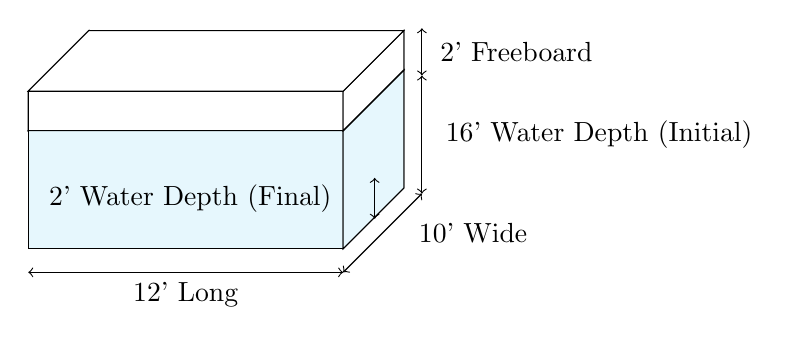
\begin{tikzpicture}

\pgfmathsetmacro{\cubexx}{4}
\pgfmathsetmacro{\cubeyy}{1.5}
\pgfmathsetmacro{\cubezz}{2}
\pgfmathsetmacro{\cubex}{4}
\pgfmathsetmacro{\cubey}{0.5}
\pgfmathsetmacro{\cubez}{2}
\pgfmathsetmacro{\cubexxx}{4}
\pgfmathsetmacro{\cubeyyy}{4}
\filldraw [fill=cyan!10!white, draw=black] (0,-\cubey,0) -- ++(-\cubexx,0,0) -- ++(0,-\cubeyy,0) -- ++(\cubexx,0,0) -- cycle ;
\filldraw [fill=cyan!0!white, draw=black] (0,-\cubey,0) -- ++(0,0,-\cubezz) -- ++(0,-\cubeyy,0) -- ++(0,0,\cubezz) -- cycle;
\filldraw [fill=cyan!10!white, draw=black] (0,-\cubey,0) -- ++(0,0,-\cubezz) -- ++(0,-\cubeyy,0) -- ++(0,0,\cubezz) -- cycle;
%\filldraw [fill=cyan!10!white, draw=black] (0,-\cubey,0) -- ++(-\cubexx,0,0) -- ++(0,0,-\cubezz) -- ++(\cubexx,0,0) -- cycle;
%%%\draw (0,-0.5,0) -- ++(-\cubex,0,0) -- ++(0,-\cubey,-\cubez) -- ++(\cubex,0,0) -- cycle;
\draw (-\cubex,0,0) -- ++(0,0,-\cubez) -- ++(0,-\cubey,0) -- ++(0,0,\cubez) -- cycle;
\draw (0,-\cubey,0) -- ++(-\cubex,0,0) -- ++(0,0,-\cubez) -- ++(\cubex,0,0) -- cycle;
\filldraw [fill=white, draw=black] (0,0,0) -- ++(-\cubex,0,0) -- ++(0,-\cubey,0) -- ++(\cubex,0,0) -- cycle ;
\filldraw [fill=white, draw=black] (0,0,0) -- ++(0,0,-\cubez) -- ++(0,-\cubey,0) -- ++(0,0,\cubez) -- cycle;
\filldraw [fill=white, draw=black] (0,0,0) -- ++(0,0,-\cubez) -- ++(0,-\cubey,0) -- ++(0,0,\cubez) -- cycle;
\filldraw [fill=white, draw=black] (0,0,0) -- ++(-\cubex,0,0) -- ++(0,0,-\cubez) -- ++(\cubex,0,0) -- cycle;

%\filldraw [fill=RoyalBlue!10!white, draw=black] (0,-1.5,0) -- ++(-\cubex,0,0) -- ++(0,-\cubey,0) -- ++(\cubex,0,0) -- cycle ;

%\filldraw [fill=RoyalBlue!10!white, draw=black] (0,-1.5,0) -- ++(0,0,-\cubez) -- ++(0,-\cubey,0) -- ++(0,0,\cubez) -- cycle;



%%\draw (0,-0.5,0) -- ++(-\cubex,0,0) -- ++(0,0,-\cubez) -- ++(\cubex,0,0) -- cycle;
%%\filldraw [fill=white, draw=black] (-\cubex,0,0) -- ++(0,0,-\cubez) -- ++(0,-\cubey,0) -- ++(0,0,\cubez) -- cycle;
%%\filldraw [fill=white, draw=black] (0,-\cubey,0) -- ++(-\cubex,0,0) -- ++(0,0,-\cubez) -- ++(\cubex,0,0) -- cycle ;

\draw [<->] (-4,-2.3) -- (0,-2.3) node [midway, below] {12' Long};
\draw [<->] (1,-1.3) -- (1,.2) node [midway, midway] {\hspace{4.5cm}16' Water Depth (Initial)};
\draw [<->] (0.4,-1.62) -- (0.4,-1.1) node [midway, midway] {\hspace{-4.8cm} 2' Water Depth (Final)};
\draw [<->] (1,.8) -- (1,.2) node [midway, midway] {\hspace{2.4cm}2' Freeboard};
\draw [<->] (1,-1.3) -- (0,-2.3) node [midway, midway] {\hspace{2.3cm}10' Wide};
\end{tikzpicture}\\
Volume to be pumped=$12 \enspace ft*10 \enspace ft *(16-2)\enspace ft=1,680ft^3$\\
\vspace{0.3cm}
$\implies \dfrac{1,680\cancel{ft^3}*7.48\dfrac{\cancel{gal}}{\cancel{ft^3}}}{600\dfrac{\cancel{gal}}{min}}=\boxed{21min}$
\end{enumerate}